% ================================================================
%  DSC 208R -- Data Management for Analytics
%  Data Parallelism (Part 2): Comprehensive Review
%  Source: "Data Engineering for ML -- Data Parallelism Part 2"
% ================================================================
\documentclass[11pt]{article}

% -------------------- Packages --------------------
\usepackage[utf8]{inputenc}
\usepackage{amsmath,amssymb,amsfonts}
\usepackage{graphicx}
\usepackage{booktabs}
\usepackage{tikz}
\usetikzlibrary{positioning}
\usepackage{pgfplots}
\usepackage{enumitem}
\usepackage{listings}
\usepackage{hyperref}
\usepackage{caption}
\pgfplotsset{compat=1.17}

% -------------------- Listings --------------------
\lstset{
  basicstyle=\ttfamily\small,
  keywordstyle=\bfseries,
  commentstyle=\itshape,
  showstringspaces=false,
  frame=single,
  breaklines=true
}

% -------------------- Document --------------------
\begin{document}

\begin{center}
  {\LARGE\bfseries Data Parallelism -- Part 2}\\[2mm]
  {\large Comprehensive Review}\\[1mm]
  {\normalsize DSC 208R -- Parallel Data Processing and the Cloud}
\end{center}
\vspace{-0.6em}\hrule\vspace{0.9em}

\tableofcontents
\newpage

% ================================================================
\section{Motivation}

Large scale data applications often rent compute in the cloud.  The slides note that fixed bundles of CPUs, memory, and storage can waste resources when an application needs only some of them.  The industry answer is newer renting paradigms such as serverless Function as a Service (FaaS).:contentReference[oaicite:0]{index=0}

% ================================================================
\section{Serverless Paradigm}

\begin{itemize}[itemsep=0pt]
  \item User uploads a function plus a resource hint (CPU and DRAM).
  \item Cloud provider hides all provisioning and autoscaling.
  \item Reported cost savings can reach 10x compared to spot instances.:contentReference[oaicite:1]{index=1}
\end{itemize}

Serverless keeps the shared nothing mindset: each function call is isolated, pulls data as needed, and scales horizontally.

\subsection*{Car Analogy}

The slides compare serverless to ride sharing: no need to buy or maintain a car; pay only for miles driven.  Similarly, serverless users pay only for milliseconds of compute.

% ================================================================
\section{Example Services}

\begin{enumerate}[itemsep=0pt]
  \item \textbf{AWS Athena} -- serverless SQL querying over S3 (schema on read).:contentReference[oaicite:2]{index=2}
  \item \textbf{AWS SageMaker plus Data Lake} -- serverless ML training and prediction.:contentReference[oaicite:3]{index=3}
  \item \textbf{AWS IoT stack} -- edge devices stream data to a serverless pipeline that does inference with SageMaker Neo.:contentReference[oaicite:4]{index=4}
\end{enumerate}

% ================================================================
\section{Resource Disaggregation}

Future clouds may fully disaggregate compute, memory, and storage: every resource is network attached and can be added or removed on demand.  The slides show a diagram where new memory and CPUs are hot plugged to speed up ongoing jobs.  Research aims to make such elasticity low latency.:contentReference[oaicite:5]{index=5}

\begin{figure}[h]
  \centering
  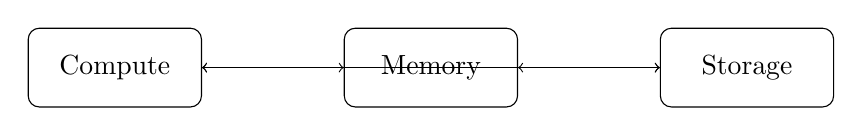
\begin{tikzpicture}[
    node/.style={draw,rounded corners,minimum width=2.2cm,minimum height=1cm},
    yshift=-0.2cm
  ]
    \node[node] (cmp) {Compute};
    \node[node,right=1.8cm of cmp] (mem) {Memory};
    \node[node,right=1.8cm of mem] (stor) {Storage};

    \draw[<->] (cmp) -- (mem);
    \draw[<->] (mem) -- (stor);
    \draw[<->] (cmp) -- (stor);
  \end{tikzpicture}
  \caption{All resources network attached and elastic.}
\end{figure}

% ================================================================
\section{Is All This Complexity Worth It?}

Cloud advantages: manageability, pay as you go cost, rapid elasticity.  
Cloud disadvantages listed in the slides:contentReference[oaicite:6]{index=6}

\begin{itemize}[itemsep=0pt]
  \item API and license complexity; need for dedicated CloudOps teams.
  \item Long term cost may exceed on premise clusters.
  \item Easy to waste money accidentally by leaving services running.
  \item Vendor lock in, privacy, security, and governance risks.
  \item Dependence on public internet and provider uptime (example 2015 AWS outage). 
\end{itemize}

Hybrid clouds remain common in enterprises, health care, and academia.

% ================================================================
\section{Cloud Adoption Surveys}

Flexera State of the Cloud surveys indicate the following trends:contentReference[oaicite:7]{index=7}

\begin{itemize}[itemsep=0pt]
  \item Public cloud spend continues to rise year over year.
  \item Many organizations use multi cloud strategies.
  \item Top challenges: controlling cost and managing cloud spend.
\end{itemize}

\begin{figure}[h]
  \centering
  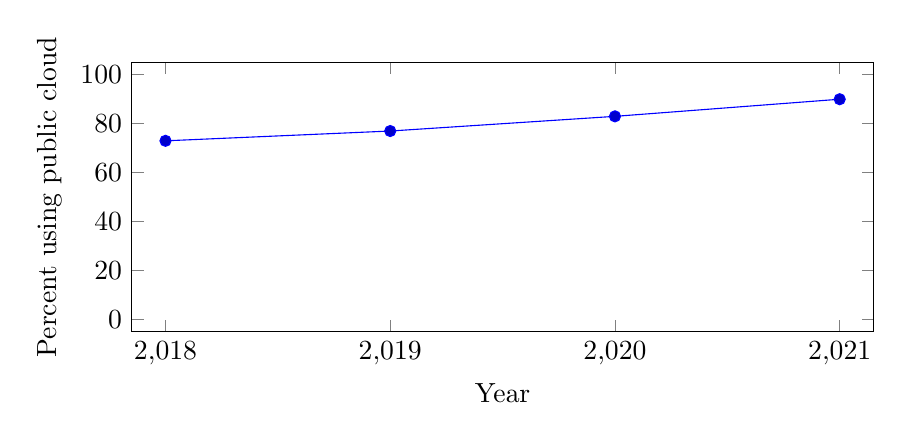
\begin{tikzpicture}
    \begin{axis}[
      width=11cm,
      height=5cm,
      xlabel=Year,
      ylabel=Percent using public cloud,
      ymin=0,ymax=100,
      xtick=data,
      ytick={0,20,40,60,80,100},
      enlargelimits=0.05
    ]
      \addplot+[mark=*] coordinates {(2018,73) (2019,77) (2020,83) (2021,90)};
    \end{axis}
  \end{tikzpicture}
  \caption{Survey trend of public cloud adoption (illustrative).}
\end{figure}

% ================================================================
\section{Pros and Cons Summary}

\begin{itemize}[itemsep=0pt]
  \item \textbf{Pros}
    \begin{itemize}[itemsep=0pt]
      \item Pay only for what you use.
      \item No cluster maintenance.
      \item Rapid scale up and down.
    \end{itemize}
  \item \textbf{Cons}
    \begin{itemize}[itemsep=0pt]
      \item Complex API landscape.
      \item Potentially higher long term cost.
      \item Risk of lock in and outages.
    \end{itemize}
\end{itemize}

% ================================================================
\section{Future Directions}

\begin{itemize}[itemsep=0pt]
  \item Fully disaggregated clouds with sub second elasticity.
  \item Better cost observability and automatic budget guards.
  \item Cross vendor orchestration to ease lock in concerns.
\end{itemize}

% ================================================================
\section*{Conclusion}

Data parallel workloads drive demand for flexible cloud resources.  Serverless and emerging disaggregation promise fine grained scaling and cost savings, but add complexity and new failure modes.  Understanding the trade offs is key when choosing between on premise, hybrid, and cloud native architectures.:contentReference[oaicite:8]{index=8}

\end{document}
